\begin{center} 
\emph{``Our lives will depend upon the decisions which we make--for decisions determine destiny.'' \\-- Thomas S. Monson}
\end{center}

\section{Introduction to Determinants}\label{sec:deter}
In a previous section, we discussed the inverse of a $2\times 2$ matrix $A = \mtx{cc}{a&b\\c&d}$:
\[A^{-1} = \dfrac{1}{ad-bc}\mtx{rr}{d&-b\\-c&a}.\] The quantity $ad-bc$ was called the \textbf{determinant} of $A$, denoted $\det A$ or $|A|$. In this chapter we work to generalize this idea for any square matrix. Our strategy will be to define determinants recursively. We will remind the reader that, unlike the previous chapter, the theory of determinants is applicable to any field. Hence, $F$ will denote an arbitrary field. \\

\begin{Def} Let $A$ be an $n\times n$ matrix. Define the $(i,j)$-\textbf{minor matrix} $A_{ij}$ to be the $(n-1)\times (n-1)$ matrix which results by removing the $i$th row and $j$th column from $A$.
\end{Def}\vs

%%Contributed by Laura Lee Fall 2018
%\begin{Exam} Let $A = \mtx{rrr}{5 & 7 & 12 \\ 0 & 3 & 4 \\ 9 & -1 & -6}$. Compute the $(1,1)-,$ $(1,2)-$, $(2,2)-$, and $(3,3)$-minor matrix.\\
%
%\[A_{11} = \mtx{rr}{3 & 4 \\ -1 & -6}, \quad A_{12} = \mtx{rr}{0 & 4 \\ 9 & -6 }, \quad A_{22} = \mtx{rr}{5 & 12 \\ 9 & -6}, \quad A_{23} = \mtx{rr}{5 & 7 \\ 9 & -1 \\},  \quad A_{33} = \mtx{rr}{5 & 7 \\  0 & 3}. \qedhere\]
%\end{Exam}\vs

\begin{Exam} Let $A = \mtx{rrr}{1&5&0\\2&4&-1\\0&-2&0}$. Compute the $(1,1)-,$ $(1,2)-$, $(2,2)-$, and $(3,3)$-minor matrix.\\

\[A_{11} = \mtx{rr}{4&-1\\-2&0}, \quad A_{12} = \mtx{rr}{2&-1\\0&0},\quad A_{22} = \mtx{rr}{1&0\\0&0}, \quad A_{33} = \mtx{rr}{1&5\\2&4}. \qedhere\]
\end{Exam}\vs

\begin{Def} Let $A = \mtx{c}{a_{ij}}$ be an $n\times n$ matrix. For $n=1$, $A = \mtx{c}{r}$ for some $r\in F$. In this case, we define $\det A = r$. For $n > 1$, let 
\begin{eqnarray*}
\det A &=& a_{11}\det A_{11} - a_{12}\det A_{12} + \ldots + (-1)^{1+n}a_{1n}\det A_{1n}\\
&=& \sum_{j=1}^n (-1)^{1+j}a_{ij}\det A_{ij}
\end{eqnarray*} The quantity $\det A$ is called the \textbf{determinant} of $A$.
\end{Def}\vs

Let $A = \mtx{cc}{a&b\\c&d}$. Then $\det A = \dtx{cc}{a&b\\c&d} = a \det A_{11} - b \det A_{12} = a\dtx{c}{d} - b\dtx{c}{c} = ad-bc,$ which agrees with our $2\times 2$ determinant from before.\\

%%Contributed by Laura Lee Fall 2018
%\begin{Exam} Compute $\det A$ for $A = \mtx{rrr}{5 & 7 & 12 \\ 0 & 3 & 4 \\ 9 & -1 & -6}$.\\
%
%\begin{eqnarray*}
%\det A &=& \dtx{rrr}{5 & 7 & 12 \\ 0 & 3 & 4 \\ 9 & -1 & -6} = 5\dtx{rr}{3 & 4 \\ -1 & -6} - 7\dtx{rr}{0 & 4 \\ 9 & -6 } + 12\dtx{rr}{0&3\\9&-1}\\
%&=& 5(3\cdot (-6) - 4\cdot(-1)) -7(0\cdot (-6) - 4\cdot 9) + 12(0\cdot (-1) - 3\cdot 9) = 5(-14) -7(-36) +12(-27)\\
%& =& -70-252-324 = \fbox{$646$}. \qedhere
%\end{eqnarray*}
%\end{Exam}\vs

\begin{Exam} Compute $\det A$ for $A = \mtx{rrr}{1&5&0\\2&4&-1\\0&-2&0}$.\\

\begin{eqnarray*}
\det A &=& \dtx{rrr}{1&5&0\\2&4&-1\\0&-2&0} = 1\dtx{rr}{4&-1\\-2&0} - 5\dtx{rr}{2&-1\\0&0} + 0\dtx{rr}{2&4\\0&-2}\\
&=& 1(4\cdot 0 - (-1)\cdot(-2)) -5(2\cdot 0 - (-1)\cdot 0) + 0 = (0-2) - 5(0) = -2. \qedhere
\end{eqnarray*}
\end{Exam}\vs

\begin{Def}  Let $A$ be an $n\times n$ matrix. Define the $(i,j)$-\textbf{cofactor} $C_{ij}$ as 
\[C_{ij} = (-1)^{i+j}\det A_{ij}.\]
\end{Def}\vs

With this notation, 
\[\det A = a_{11}C_{11} + a_{12}C_{12} + \ldots + a_{1n}C_{1n}.\]\vs

The following diagram may help you remember the plus or minus sign in the cofactors:
\[\mtx{rrrr}{+ & -& + & \cdots \\ - & + & -&  \\ + & -& + &  \\ \vdots & & &\ddots}\]\vs

\begin{Thm}[Laplace Expansion] The determinant of an $n\times n$ matrix $A = \mtx{c}{a_{ij}}$ can be computed by a cofactor expansion across any row or down any column. The cofactor expansion across the $i$th row is 
\[\det A = a_{i1}C_{i1} + a_{i2}C_{i2} + \ldots + a_{in}C_{in} = \sum_{j=1}^n a_{ij}C_{ij}.\] The cofactor expansion down the $j$th column is
\[\det A = a_{ij}C_{1j} + a_{2j}C_{2j} + \ldots + a_{nj}C_{nj} = \sum_{i=1}^n a_{ij}C_{ij}.\]
\end{Thm}\vs

\begin{Exam} Use the cofactor expansion across the third row to compute $\det A$, where $A = \mtx{rrr}{1&5&0\\2&4&-1\\0&-2&0}$.

\begin{eqnarray*}
\det A &=& \dtx{rrr}{1&5&0\\2&4&-1\\0&-2&0} = 0\dtx{rr}{5&0\\4&-1} - (-2)\dtx{rr}{1&0\\2&-1} + 0\dtx{rr}{1&5\\2&4}\\
&=& 2\dtx{rr}{1&0\\2&-1} = 2(-1-0) = \fbox{$-2$}.
\end{eqnarray*}
\end{Exam}

\begin{Exam} Compute $\det A$, where $A = \mtx{rrrrr}{3&-7&8&9&-6\\0&2&-5&7&3\\0&0&1&5&0\\0&0&2&4&-1\\0&0&0&-2&0}$.\\

We will expand across the leftmost column to maximize the number of zero coefficients.
\begin{eqnarray*}
\dtx{rrrrr}{3&-7&8&9&-6\\0&2&-5&7&3\\0&0&1&5&0\\0&0&2&4&-1\\0&0&0&-2&0} &=& 3\dtx{rrrr}{2&-5&7&3\\0&1&5&0\\0&2&4&-1\\0&0&-2&0} = 6\dtx{rrr}{1&5&0\\2&4&-1\\0&-2&0}\\
&=& 6\left(\dtx{rr}{4&-1\\-2&0} - 2\dtx{rrrr}{5&0\\-2&0}\right)=6(-2+0) = \fbox{$-12$}
\end{eqnarray*}
\end{Exam}

The matrix in the last example is nearly triangular. The method in that example is easily adapted to prove the following.\\

\begin{Thm} If $A$ is a triangular $n\times n$ matrix, then $\det A$ is the product of the entries on the main diagonal.
\end{Thm}

\begin{multicols}{2}
\begin{Thm} If $A$ is a $2\times 2$ matrix over $\R$ or $\C$, the area of the parallelogram determined by the columns of $A$ is $|\det A|$. If $A$ is $3\times 3$, the volume of the parallelepiped determined by the columns of $A$ is $|\det A|$. The higher dimensional analogues also hold.
\end{Thm}
\begin{center}
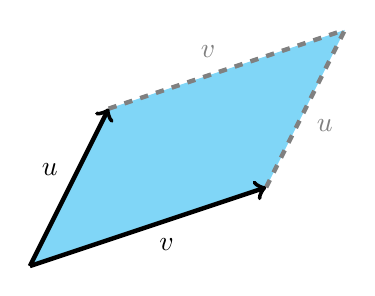
\begin{tikzpicture}
\fill[cyan!50!white] (0,0) -- (1,2) -- (4,3) -- (3,1) -- cycle;
\draw[dashed, ultra thick, gray] (1,2) -- (4,3) node[midway, above left] {$\bb v$};
\draw[dashed, ultra thick, gray] (3,1) -- (4,3) node[midway, below right] {$\bb u$}; 
\draw[->, ultra thick] (0,0) -- (3,1) node[midway, below right] {$\bb v$};
\draw[->, ultra thick] (0,0) -- (1,2) node[midway, above left] {$\bb u$};
%\draw[->, ultra thick, red] (0,0) -- (4,3) node[midway, above, yshift = -5] {\rotatebox{35}{$\bb u + \bb v$}};
\end{tikzpicture}
\end{center}
\end{multicols}\vs
%\begin{proof}
%We will prove the statement for the general case of $n\times n$. If $\det A = 0$, then the column vectors are linearly dependent and the hyper-parallelepiped spanned by them is one dimension too small. Thus, the hyper-volume is also zero. If $\det A \neq 0$, then the column vectors are linearly independent and hence span all dimensions. This hyper-parallelepiped can be sheared into a rectangular hyper-prism, that is, all angles are right. A shearing matrix $S$ is unit triangular matrices and hence have determinant equal to 1. Likewise, by permuting rows, the matrix corresponding to the rectangular hyper-prism can be transformed into a diagonal matrix $D$ by multiplying by the associated permutation matrix $P$. Then $|\det(D)| = |\det(A)| $, which is the absolute value  product of the diagonal entries. On the other hand, the hyper-volume of a hyper-prism is the product of all the lengths, which are the absolute values of the diagonal entries of $D$.
%\end{proof}\vs

\begin{Exam} Calculate the area of the parallelogram determined by the points $(-2,-2)$, $(0,3)$, $(4,-1)$, and $(6,4)$.\\

We begin by translating the parallelogram such that $(-2,-2)$ is moved to the origin. This translation does not affect the area. We now consider the parallelogram with vertices $(0,0)$, $(2,5)$, $(6,1)$, and $(8,6)$. Note that this parallelogram is the one spanned by $(2,5)$ and $(6,1)$. Therefore, 
\[\text{Area} = \text{abs}\dtx{rr}{2&6\\5&1}= |2-30| = \fbox{$28$}.\qedhere\]
\end{Exam}\vs

%\section{Properties of Determinants}
%\begin{Thm}\label{product} If $A$ and $B$ are $n \times n$ matrices, then $\det(AB) = \det(A)\det(B)$.\end{Thm}\vs
%
%\begin{Exam} Let $A = \mtx{rr}{6&1\\3&2}$ and $B =\mtx{rr}{4&3\\1&2}$. Then $\det A = 6(2)-1(3) = 9$ and $\det B = 4(2)-3(1)=5$. Thus, $\det(A)\det(B) = \fbox{$45$}$. On the other hand, 
%\[AB = \mtx{rr}{6&1\\3&2}\mtx{rr}{4&3\\1&2} = \mtx{rr}{25 & 20\\ 14&13}.\] Thus, $\det(AB) = 25(13)-20(14) = 325-280= \fbox{$45$}$. 
%\end{Exam}\vs
%
%%%%%%%%%%%%%%%%%% Exercises %%%%%%%%%%%%%%%%%%%
\startExercises{deter}
\noindent For Exercises \ref{exer:minorstart}-\ref{exer:minorstop}, for the matrix $A = \mtx{rrr}{ 5 & 7 & 12 \\ 0 & 3 & 4 \\  9 & -1 & -6}$, find the given minor.
\begin{enumerate}[!HW!, start=1]
\begin{multicols}{5}
\item\label{exer:minorstart} $A_{22}$ %Laura Lee
\item $A_{33}$ %Laura Lee
\item $A_{11}$ %Laura Lee
\item $A_{23}$ %Laura Lee
\item\label{exer:minorstop} $A_{12}$ %Laura Lee
\end{multicols}
\end{enumerate}

\noindent For Exercises \ref{exer:minorspadestart}-\ref{exer:minorspadestop}, for the matrix $B = \mtx{rrrr}{1 & 2 & 3 & 4 \\ 0 & -2 & -1 & 3 \\ 1 & 1 & 3 & 6\\ 7 & -4 & 8 & 0}$, find the given minor.
\begin{enumerate}[!HW!, label=$\spadesuit$ \arabic*., ref=\arabic*]
\begin{multicols}{5}
\item\label{exer:minorspadestart} $B_{11}$
\item $B_{13}$
\item $B_{31}$
\item $B_{33}$
\item\label{exer:minorspadestop} $B_{34}$
\end{multicols}
\end{enumerate}

%NEW
\noindent For Exercises \ref{exer:minorboringstart}-\ref{exer:minorboringstop}, for the matrix $C = \mtx{rrrr}{1&2&3&4\\0&5&3&-1\\-2&4&0&-4\\-1&3&2&5}$, find the given minor.
\begin{enumerate}[!HW!]
\begin{multicols}{3}
\item\label{exer:minorboringstart} $C_{22}$
\item $C_{23}$
\item\label{exer:minorboringstop} $C_{42}$
\end{multicols}
\end{enumerate}

\noindent For Exercises \ref{exer:minorcomplexstart}-\ref{exer:minorcomplexstop}, for the matrix $D = \mtx{cccc}{i&3i-2&2+5i&7-i\\3+i&4&7i-5&9-3i\\2+3i&5i-1&1+9i&4+5i\\7+2i&i-3&2+4i&1+2i}$, find the given minor.
\begin{enumerate}[!HW!]
\begin{multicols}{3}
\item\label{exer:minorcomplexstart} $D_{24}$%Malcolm Hanks
\item $D_{33}$%Malcolm Hanks
\item\label{exer:minorcomplexstop} $D_{14}$%Malcolm Hanks
\end{multicols}
\end{enumerate}

\noindent For Exercises \ref{exer:determinantstart}-\ref{exer:determinantstop}, compute the determinant of the matrix.
\begin{enumerate}[!HW!, label=$\spadesuit$ \arabic*., ref=\arabic*]
\begin{multicols}{3}
\item\label{exer:determinantstart} $\dtx{rr}{1 & 2 \\ 3 & 4}$
\itemspade $\dtx{cc}{i & 1+i \\ 2-i & 3-4i}$
\itemspade \mbox{$\dtx{rr}{3 & 2\\ 1 & 5} \pmod 7$}  
\end{multicols}
\end{enumerate}
\begin{enumerate}[!HW!]
\begin{multicols}{3}
\itemspade $\dtx{rrr}{1 & 2 & -1 \\ -1 & 0 & 2\\ 3 & 5 & 1}$ 
\itemspade $\dtx{rrr}{1 & 2 & 3\\ 3 & -2 & 5 \\ 0 & 0 & 2}$ 
\itemspade \mbox{$\dtx{rrr}{2 & 0 & 0\\ 3 & 1 & 0\\ 4 & 3 & 4} \pmod 5$} 
\end{multicols}\pagebreak
\begin{multicols}{3}
\itemspade \mbox{$\dtx{rrrr}{1 & 1 & 2 & 4 \\ 0 & 1 & 1 & 3 \\ 0 & 0 & 2 & 4 \\ 1 & 2  & 3 & 4} \pmod 5$}
\itemspade \mbox{$\dtx{rrrrr}{1 & 0 & 0 & 0 &0 \\ 0 & 0 & 0 & 1 &0 \\ 0 &0 & 1 & 0 & 0 \\ 0 &0 & 1 & 0 & 0 \\ 0 &0 & 0 &0 &1} \pmod 2$}
\item\label{exer:determinantstop} $\dtx{rrrr}{5&4&4&2\\2&4&6&8\\0&1&2&3\\3&3&3&9}$ %Shelby Bartlett
\end{multicols}
\end{enumerate}

\begin{enumerate}[!HW!]
    \item Compute $\det(A)(\bb u\cdot \bb v)$ if:
    \[A = \mtx{cc}{\pi^2&e\\5&\sqrt{\pi}},\quad \bb u = \mtx{c}{5e^3\\1\\\pi},\quad \bb v = \mtx{c}{e^{-2}\\0\\\sqrt{\pi^3}}.\] %Da Huo
\end{enumerate}

\noindent For Exercises \ref{exer:detervolumestart}-\ref{exer:detervolumestop}, compute the area, volume, or hyper-volume of the parallelogram, parallelepiped, or hyper-parallelepiped spanned by the given set of vectors. 
\begin{enumerate}[!HW!, label=$\spadesuit$ \arabic*., ref=\arabic*]
\begin{multicols}{3}
\item\label{exer:detervolumestart} $\left\{\vr{1 \\ 2}, \vr{3\\2}\right\}$ 
\itemspade $\left\{\vr{1 \\ 2 \\ 3}, \vr{4\\8\\2}, \vr{-2 \\ 3 \\ 7}\right\}$
\item\label{exer:detervolumestop} $\left\{\vr{1 \\ 2 \\ 3 \\ 4}, \vr{1 \\ 0 \\ 0 \\ 2}, \vr{0 \\ 0 \\ 1 \\-2}, \vr{2\\-3\\4\\5}\right\}$
\end{multicols}
\end{enumerate}


%%%%%%%%%%%%%%%%%%% Footnotes %%%%%%%%%%%%%%%%%%%
 \mbox{}\vfill
 
\pagebreak